\begin{surferPage}{Eine $A_3^{--}$ Singularität}
Direkt an der Gleichung
    \[x^4-y^2-z^2=0\]
    kann man ablesen, dass diese Fläche der vorigen (nämlich $A_3^{+-}$ mit
    der 
    Gleichung $x^4+y^2-z^2$) sehr ähnlich ist. 
    Schön sieht man dies auch, wenn man sich beide Flächen gemeinsam in einem
    Bild veranschaulicht; der Schnitt mit der Ebene $y=0$ ist identisch:  
    \vspace*{-0.5em}
    \begin{center}
      \begin{tabular}{c@{\qquad}c}
        \begin{tabular}{@{}c@{}}
          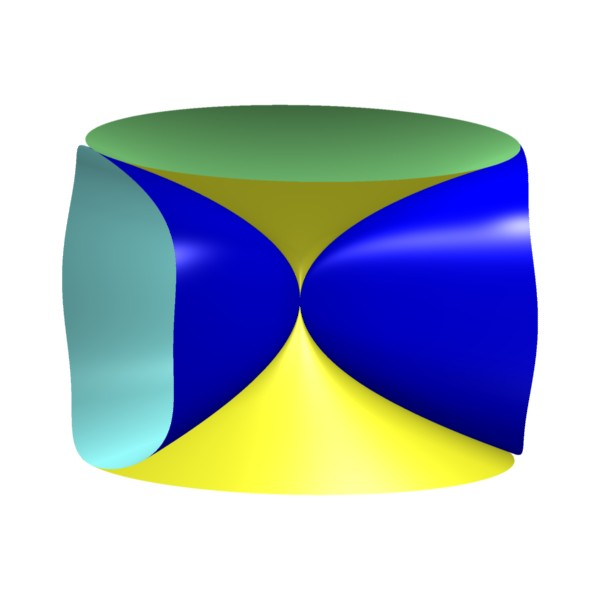
\includegraphics[width=1.6cm]{../../common/images/A3pmA3mm}
        \end{tabular}
        &
        \begin{tabular}{@{}c@{}}
          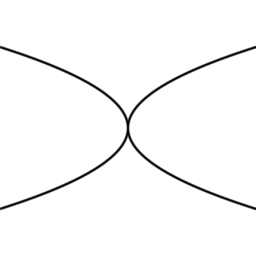
\includegraphics[width=1.6cm]{../../common/images/A3pm_cut}
        \end{tabular}
      \end{tabular}
    \end{center}
    \vspace*{-0.1cm}
    Auch diese $A_k$-Singularität lässt sich in $\lfloor\frac{k+1}{2}\rfloor$
    Doppelkegel deformieren; hier ergeben sich, da $k=3$, zwei $A_1$-en: 
%    \dontshow{
    % 
    \begin{center}
      \vspace*{-0.1cm}
      \begin{tabular}{@{}c@{\quad}c@{\quad}c@{}}
        \begin{tabular}{@{}c@{}}
          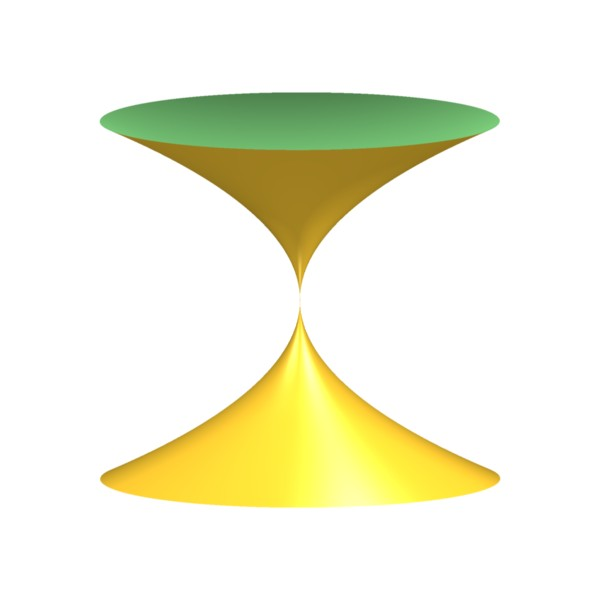
\includegraphics[width=1.6cm]{../../common/images/A3mm_0}
        \end{tabular}
        &
        \begin{tabular}{@{}c@{}}
          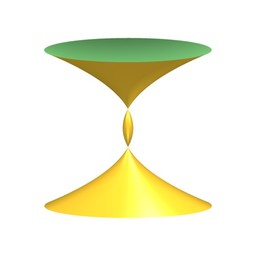
\includegraphics[width=1.6cm]{../../common/images/A3mm_1}
        \end{tabular}
        &
        \begin{tabular}{@{}c@{}}
          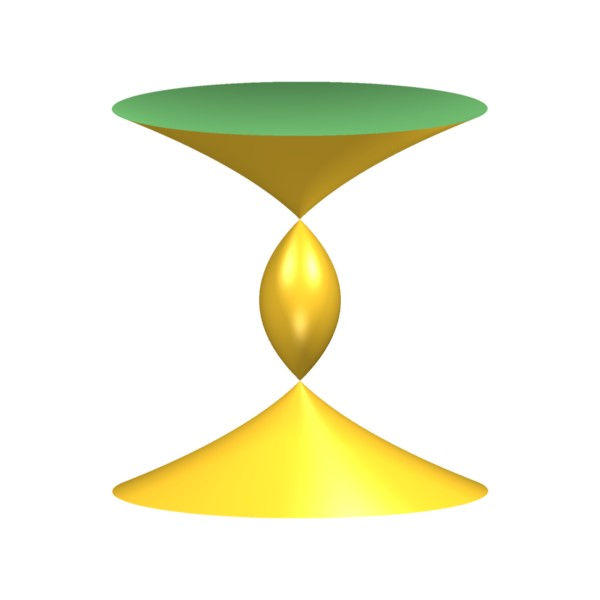
\includegraphics[width=1.6cm]{../../common/images/A3mm_2}
        \end{tabular}
      \end{tabular}
    \end{center}
%    }
      \vspace*{-0.2cm}
    Man kann diese Störung der $A_3^{--}$ Singularität 
    z.B.\ mit folgender Formel erreichen: 
    \[\bigl(x-\frac12 a^2\bigr)^2\bigl(x+\frac12 a^2\bigr)^2-y^2-z^2.\]
 
\end{surferPage}

